\documentclass[]{article}
\usepackage[czech]{babel}
\usepackage[utf8]{inputenc}
\usepackage{float}
\usepackage{subfig,graphicx}
\usepackage{array}
\usepackage{color}
\usepackage{makecell}

\newcommand{\ptheory}{$\Psi$-theory }

\begin{document}

\title{Kapitola 6: Aplikace metody}
\author{Bc. Štěpán Heller}
\date{\today}
\maketitle

\section{Úvod}
V předchozí kapitole byl představen návrh metody pro vytváření BPMN modelů za použití Enterprise ontology, \ptheory a metodologie DEMO. Cílem metody má být umožnit vytvářet BPMN modely, které budou vždy \textit{konzistentní}, \textit{kompletní} a \textit{jednoznačné}.

V této sekci je navržená metoda aplikována po jednotlivých krocích na konkrétní příklad a na závěr jsou diskutovány výsledky. Aplikace kroků 1, 2, 3 a 6 vycházejí z analogických postupů popsaných v \cite{Dietz2006}.

\section{Aplikace metody}
\subsection{Krok 1: Získání textového popisu procesu}
Pro demonstraci metody použijeme výňatek (první fázi) z příkladu Pizzeria Mama Mia z \cite{Dietz2006}, kterou používá rovněž \cite{VanNuffel2009}. Popis situace je následující:
\begin{quote}
Zákazníci si objednávají přímo v pizzerii, nebo si s objednávkou zavolají. V obou případech Mia zapíše jméno zákazníka, objednávku a celkovou cenou na objednávkový formulář. Na pultu leží seznam nabízených pizz a jejich cen. Mia obvykle nové menu vytváří během své každoroční dovolené. V případě telefonické objednávky také zaznamenává telefonní číslo. Navíc zopakuje objednávku a informuje zákazníka o ceně a předpokládaném čase, než bude pizza připravena. Pokud je to nutné sdělí také zákazníkovi akutální nabídku pizz. Objednávkové formuláře mají sériové číslo a jsou vyhotoveny ve dvou kopiích – v růžové a bílé kopii. Mia posune růžový formulář přes okno ve zdi do kuchyně, kde se Mario stará o pečení pizzy. Bílou kopii si Mia nechá za pultem. Jakmile Mario dokončil objednávku, podá pizzy v krabicích přes okno Mie, včetně růžové kopie objednávky. Mia pak hledá odpovídající bílou kopii, kterou podá spolu s krabicemi zákazníkovi a čeká na platbu. Může se stát, že Mario není schopen objednávce vyhovět kvůli chybějícím ingrediencím. V takovém případě prostrčí hlavu oknem ve zdi a upozorní Miu na problém. Vrátí také růžovou kopii. Pokud je zákazník přítomen v obchodě, Mia se s ním poradí, jak objednávku upravit. V případě, že zákazník není přítomen, což je častější případ, Mia změní objednávku podle vlastního uvážení. To někdy vede k vášnivým debatám v pizzerii, když si zákazník přijde pro svojí objednávku. Díky Miině temperamentu vždycky nakonec dojde k dohodě, která není nevýhodná pro ni.
\footnote{Customers address themselves to the counter of the pizzeria or make a telephone call. In both cases Mia writes down the name of the customer, the ordered items, and the total price on an order form. On the counter lies a plasticized list of the available pizza’s and their prices. Usually she pro- duces this list every year during their holiday. In case of an order by telephone she also records the telephone number. Moreover, she repeats the ordered items and informs the customer about the price and the expected time that the order will be ready. If necessary, she also tells the customer the assortment of pizzas. The order forms have a serial number and are produced in duplicate: a white and a pink copy. Mia shifts the pink one through a hatch in the wall to the kitchen, where Mario takes care of baking the pizzas. She keeps the white copy behind the counter. As soon as Mario has finished an order, he shifts the pizzas in boxes through the same hatch to Mia, including the pink order copy. Mia then seeks the matching white copy, hands it together with the boxes over to the customer, and waits for payment. It may happen that Mario is not able to fulfill an order completely because of missing ingredients. In such a case he puts his head through the hatch and notifies Mia of the problem. He then also returns the pink copy. If the customer is present in the shop, she confers with him or her what to do about it, and modifies the order. If the customer is not present, which is mostly the case for tele- phonic orders, she modifies the order to her own discretion. This leads sometimes to vigorous debates in the pizzeria when the customer comes for taking away the order. Thanks to Mia’s temperament she always comes to an agreement that is not disadvantageous for her.}
\end{quote}

\subsection{Krok 2: Aplikace distinkčního axiomu}
V rámci druhého kroku navržené metody je třeba na prostý textový proces aplikovat distinkční axiom, neboli provést \textit{Performa-Informa-Forma analýzu}. Tu provádíme tak, že pročítáme text a označujeme barevně (Performa červeně, Informa modře, Forma zeleně) aktivity v popisu. Vznikne nám tak text, ze kterého lze jednoduše barevně odlišit červené Performa aktivity, které budeme dále analyzovat.

Znovu se na tomto místě sluší zopakovat, že je naprosto přirozené, že některé aktivity bude zprvu obtížné barevně klasifikovat. V takovém případě je vhodné se pokusit odhadnout zařazení aktivity a po aplikaci dalších kroků a získání přesnějšího náhledu na problém své rozhodnutí případně přehodnotit. Výsledek po aplikaci druhého kroku vidíme níže:

\begin{quote}
Zákazníci si \textcolor{red}{objednávají} přímo v pizzerii, nebo si s objednávkou zavolají. V obou případech Mia \textcolor{green}{zapíše} \textcolor{blue}{jméno zákazníka, objednávku a celkovou cenou} na \textcolor{green}{objednávkový formulář}. Na pultu \textcolor{green}{leží seznam} \textcolor{blue}{nabízených pizz a jejich cen}. Mia obvykle nové menu \textcolor{red}{vytváří} během své každoroční dovolené. V případě telefonické objednávky také \textcolor{green}{zaznamenává} \textcolor{blue}{telefonní číslo}. Navíc \textcolor{blue}{zopakuje objednávku} a \textcolor{blue}{informuje zákazníka o ceně a předpokládaném čase}, než bude pizza připravena. Pokud je to nutné \textcolor{blue}{sdělí také zákazníkovi akutální nabídku pizz}. 

Objednávkové formuláře mají sériové číslo a jsou vyhotoveny ve dvou kopiích – v růžové a bílé kopii. Mia \textcolor{green}{posune růžový formulář} přes okno ve zdi do kuchyně, kde se Mario stará o \textcolor{red}{pečení pizzy}. Bílou kopii si Mia nechá za pultem. Jakmile Mario \textcolor{red}{dokončil objednávku}, \textcolor{green}{podá} pizzy v krabicích přes okno Mie, včetně \textcolor{green}{růžové kopie objednávky}. Mia pak hledá odpovídající bílou kopii, kterou \textcolor{green}{podá} spolu s krabicemi \textcolor{green}{zákazníkovi} a čeká na \textcolor{red}{platbu}. 

Může se stát, že Mario není schopen objednávce vyhovět kvůli chybějícím ingrediencím. V takovém případě prostrčí hlavu oknem ve zdi a \textcolor{blue}{upozorní Miu na problém}. \textcolor{green}{Vrátí také růžovou kopii}. Pokud je zákazník přítomen v obchodě, Mia se s ním \textcolor{red}{poradí}, jak objednávku upravit. V případě, že zákazník není přítomen, což je častější případ, Mia \textcolor{red}{změní objednávku podle vlastního uvážení}. To někdy vede k vášnivým debatám v pizzerii, když si zákazník přijde pro svojí objednávku. Díky Miině temperamentu vždycky nakonec \textcolor{red}{dojde k dohodě}, která není nevýhodná pro ni.
\end{quote}

\subsection{Krok 3: Aplikace operačního axiomu}
Jak již bylo řečeno v předchozí sekci, v rámci aplikace třetího kroku pracujeme pouze s Perfroma aktivitami, které jsme označili červeně. Úkolem je nyní klasifikovat červeně označené aktivity jako C-acty, C-facty, P-acty a P-facty za použití různých druhů závorek popsaných v sekci \ref{sec:st3_opax}. Výsledek můžeme vidět na textu níže:

\begin{quote}
[\underline{Zákazníci}] si (\underline{\textcolor{red}{objednávají}}) přímo v pizzerii, nebo si s objednávkou zavolají. V obou případech [\underline{Mia}] \textcolor{green}{zapíše} \textcolor{blue}{jméno zákazníka, objednávku a celkovou cenou} na \textcolor{green}{objednávkový formulář}. Na pultu \textcolor{green}{leží seznam} \textcolor{blue}{nabízených pizz a jejich cen}. Mia obvykle nové menu $<$\underline{\textcolor{red}{vytváří}}$>$ během své každoroční dovolené. V případě telefonické objednávky také \textcolor{green}{zaznamenává} \textcolor{blue}{telefonní číslo}. Navíc \textcolor{blue}{zopakuje objednávku} a \textcolor{blue}{informuje zákazníka o ceně a předpokládaném čase}, než bude pizza připravena. Pokud je to nutné \textcolor{blue}{sdělí také zákazníkovi akutální nabídku pizz}. 

Objednávkové formuláře mají sériové číslo a jsou vyhotoveny ve dvou kopiích – v růžové a bílé kopii. [\underline{Mia}] \textcolor{green}{(\underline{posune}) růžový formulář} přes okno ve zdi do kuchyně, kde se [\underline{Mario}] stará o \textcolor{red}{$<$\underline{pečení}$>$ pizzy}. Bílou kopii si Mia nechá za pultem. Jakmile Mario \textcolor{red}{$<$\underline{dokončil}$>$ objednávku}, \textcolor{green}{(\underline{podá}} pizzy v krabicích přes okno Mie, včetně \textcolor{green}{\underline{růžové kopie} \underline{objednávky})}. Mia pak hledá odpovídající bílou kopii, kterou \textcolor{green}{(\underline{podá}} spolu s krabicemi \textcolor{green}{\underline{zákazníkovi})} a čeká na \textcolor{red}{$<$\underline{platbu}$>$}. 

Může se stát, že Mario není schopen objednávce vyhovět kvůli chybějícím ingrediencím. V takovém případě prostrčí hlavu oknem ve zdi a \textcolor{blue}{upozorní Miu na problém}. \textcolor{green}{Vrátí také růžovou kopii}. Pokud je zákazník přítomen v obchodě, [\underline{Mia}] se s [\underline{ním}] \textcolor{red}{(\underline{poradí})}, jak objednávku upravit. V případě, že zákazník není přítomen, což je častější případ, Mia \textcolor{red}{(\underline{změní objednávku}) podle vlastního uvážení}. To někdy vede k vášnivým debatám v pizzerii, když si zákazník přijde pro svojí objednávku. Díky Miině temperamentu vždycky nakonec \textcolor{red}{dojde k (\underline{dohodě})}, která není nevýhodná pro ni.
\end{quote}

Můžeme vidět, že jsme závorkami a podtržením označili i aktivity, které jsme v kroku 2 označili modře nebo zeleně. Není na tom nic špatného a při analýze procesu je zcela přirozené neustále zpřesňovat své závěry. Můžeme se díky tomu vrátit ke krokům 2 a 3 a upravit je tak, aby text, který jsme označili závorkami byl vždy červený. Závěr třetího kroku by tedy mohl vypadat nakonec takto:

\begin{quote}
[\underline{Zákazníci}] si (\underline{\textcolor{red}{objednávají}}) přímo v pizzerii, nebo si s objednávkou zavolají. V obou případech [\underline{Mia}] \textcolor{green}{zapíše} \textcolor{blue}{jméno zákazníka, objednávku a celkovou cenou} na \textcolor{green}{objednávkový formulář}. Na pultu \textcolor{green}{leží seznam} \textcolor{blue}{nabízených pizz a jejich cen}. Mia obvykle nové menu $<$\underline{\textcolor{red}{vytváří}}$>$ během své každoroční dovolené. V případě telefonické objednávky také \textcolor{green}{zaznamenává} \textcolor{blue}{telefonní číslo}. Navíc \textcolor{blue}{zopakuje objednávku} a \textcolor{blue}{informuje zákazníka o ceně a předpokládaném čase}, než bude pizza připravena. Pokud je to nutné \textcolor{blue}{sdělí také zákazníkovi akutální nabídku pizz}. 

Objednávkové formuláře mají sériové číslo a jsou vyhotoveny ve dvou kopiích – v růžové a bílé kopii. [\underline{Mia}] \textcolor{red}{(\underline{posune}) růžový formulář} přes okno ve zdi do kuchyně, kde se [\underline{Mario}] stará o \textcolor{red}{$<$\underline{pečení}$>$ pizzy}. Bílou kopii si Mia nechá za pultem. Jakmile Mario \textcolor{red}{$<$\underline{dokončil}$>$ objednávku}, \textcolor{red}{(\underline{podá}} pizzy v krabicích přes okno Mie, včetně \textcolor{red}{\underline{růžové kopie} \underline{objednávky})}. Mia pak hledá odpovídající bílou kopii, kterou \textcolor{red}{(\underline{podá}} spolu s krabicemi \textcolor{red}{\underline{zákazníkovi})} a čeká na \textcolor{red}{$<$\underline{platbu}$>$}. 

Může se stát, že Mario není schopen objednávce vyhovět kvůli chybějícím ingrediencím. V takovém případě prostrčí hlavu oknem ve zdi a \textcolor{blue}{upozorní Miu na problém}. \textcolor{green}{Vrátí také růžovou kopii}. Pokud je zákazník přítomen v obchodě, [\underline{Mia}] se s [\underline{ním}] \textcolor{red}{(\underline{poradí})}, jak objednávku upravit. V případě, že zákazník není přítomen, což je častější případ, Mia \textcolor{red}{(\underline{změní objednávku}) podle vlastního uvážení}. To někdy vede k vášnivým debatám v pizzerii, když si zákazník přijde pro svojí objednávku. Díky Miině temperamentu vždycky nakonec \textcolor{red}{dojde k (\underline{dohodě})}, která není nevýhodná pro ni.
\end{quote}

\subsection{Krok 4: Zápis nalezených transakcí a jejich parametrů}
Pro snazší práci v dalších krocích i případnou budoucí automatizaci si identifikované transakce (korespondující s P-acty a P-facty, které jsme označili \uv{špičatými závorkami}). Jedná se o:

\begin{itemize}
\item Vyřízení objednávky $O$ (tato transakce nemá v textovém popisu žádný korespondující P-act nebo P-fact, ale její existenci odvodíme z identifikovaného C-actu v podobě objednávání pizzy zákazníky)
\item Příprava objednávky $O$ 
\item Platba objednávky $O$ 
\end{itemize}

Identifikované transakce a jejich parametry zapíšeme do tabulek \ref{tab:t01_param}, \ref{tab:t02_param} a \ref{tab:t03_param}.

\begin{table} [H] \centering
\begin{tabular}{|>{\bfseries} l| | c |}
\hline
  ID transakce & T01 \\
\hline
  Název transakce & Vyřízení objednávky $O$  \\
\hline
  Výsledek transakce & Objednávka $O$ byla vyřízena \\
\hline
  Initiator & Zákazník \\
\hline
  Executor & Mia \\
\hline
\hline
  Request & Zavolání s objednávkou nebo objednání osobně \\
\hline
  Promise & \makecell{Potvrzení s cenou a časem vyhotovení (telefonicky), \\ \textit{chybí v popisu (osobní odběr)}}\\
\hline
  State & Pizza předána zákazníkovi \\
\hline
  Accept & \textit{chybí v popisu} \\
\hline
\hline
  Decline &  \textit{chybí v popisu} \\
\hline
  Reject & \textit{chybí v popisu} \\
\hline
\hline
  Revoke request & \textit{chybí v popisu} \\
\hline
  Revoke promise & \textit{chybí v popisu} \\
\hline
  Revoke state & \textit{chybí v popisu} \\
\hline
  Revoke accept & \textit{chybí v popisu} \\
\hline
\end{tabular}
\caption{Parametry transakce T01}
\label{tab:t01_param}
\end{table}

\begin{table} [H] \centering
\begin{tabular}{|>{\bfseries} l| | c |}
\hline
  ID transakce & T02 \\
\hline
  Název transakce & Příprava objednávky $O$  \\
\hline
  Výsledek transakce & Objednávka $O$ byla připravena \\
\hline
  Initiator & Mia \\
\hline
  Executor & Mario \\
\hline
\hline
  Request & Posunutí objednávkového formuláře do kuchyně \\
\hline
  Promise &  \textit{chybí v popisu} \\
\hline
  State & Podání pizz přes okno Mie \\
\hline
  Accept & \textit{chybí v popisu} \\
\hline
\hline
  Decline &  Upozornění Mii na chybějící ingredience \\
\hline
  Reject & \textit{chybí v popisu} \\
\hline
\hline
  Revoke request & \textit{chybí v popisu} \\
\hline
  Revoke promise & \textit{chybí v popisu} \\
\hline
  Revoke state & \textit{chybí v popisu} \\
\hline
  Revoke accept & \textit{chybí v popisu} \\
\hline
\end{tabular}
\caption{Parametry transakce T02}
\label{tab:t02_param}
\end{table}

\begin{table} [H] \centering
\begin{tabular}{|>{\bfseries} l| | c |}
\hline
  ID transakce & T03 \\
\hline
  Název transakce & Platba  \\
\hline
  Výsledek transakce & Objednávka $O$ byla zaplacena \\
\hline
  Initiator & Mia \\
\hline
  Executor & Zákazník \\
\hline
\hline
  Request & \makecell{Podání krabic s objednávkou a objednávkovým\\ formulářem zákazníkovi} \\
\hline
  Promise &  \textit{chybí v popisu} \\
\hline
  State & \textit{chybí v popisu} \\
\hline
  Accept & \textit{chybí v popisu} \\
\hline
\hline
  Decline &  \textit{chybí v popisu} \\
\hline
  Reject & \textit{chybí v popisu} \\
\hline
\hline
  Revoke request & \textit{chybí v popisu} \\
\hline
  Revoke promise & \textit{chybí v popisu} \\
\hline
  Revoke state & \textit{chybí v popisu} \\
\hline
  Revoke accept & \textit{chybí v popisu} \\
\hline
\end{tabular}
\caption{Parametry transakce T03}
\label{tab:t03_param}
\end{table}

Ve vyplněných tabulkách můžeme vidět, že v nich valná část transakčních kroků chybí, protože nejsou uvedeny v textovém popisu případu Pizzerie Mama Mia. Takový případ bude nastávat v reálném světě velmi často a jeho ideálním řešení je návrat do kroku 1 a získání chybějících informací od vlastníků procesu a dalších zasvěcených osob.

Jelikož případ Pizzerie Mama Mia popsal v \cite{Dietz2006} pan profesor Dietz, zeptat se ho nemůžeme. Pro aplikaci dalších kroků nám však stačí i takovýto neúplný popis. Ve výsledném BPMN modelu však pojmenujeme všechny transakční kroky dle názvů, které nesou v základním transakčním vzoru a ne jmény reálných aktivit, které jsme identifikovali.

\subsection{Krok 5: Aplikace kompozičního axiomu}
Dalším krokem je aplikování kompozičního axiomu a odhalení struktury v jaké jsou jednotlivé transakce navzájem propojeny. Jinými slovy musíme zjistit, která transakce je kořenová a z jakých transakcí se tato transakce skládá, což nám pomůže určit, v jakém pořadí jsou transakce prováděny.

Tento krok není možné udělat jinak, než že se vrátíme k textovému popisu, který je výsledkem kroku 3 a hledáme náznaky závislostí mezi transakcemi a pořadí v jakém jsou tyto transakce vykonávány. Zjištění pak vyjádříme v jednoduchém grafu. Výsledek pro případ Pizzerie Mama Mia můžeme vidět níže na obrázku \ref{fig:result_structure_chart}:

\begin{figure}[H]\centering
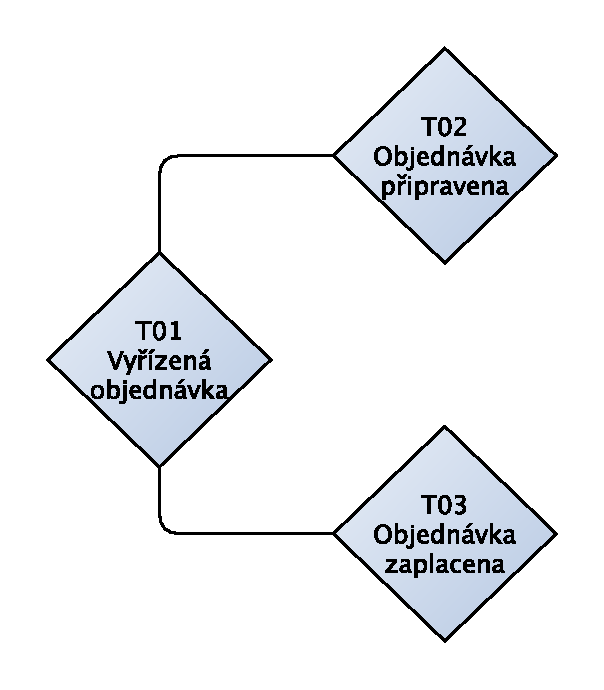
\includegraphics[scale=0.75]{obrazky/result-structure-chart-pizzeria}
\caption{Struktura závislosti transakcí v případu Pizzerie Mama Mia}
\label{fig:result_structure_chart}
\end{figure}

\subsection{Krok 6: Vytvoření DEMO modelů}
V předposledním kroku navržené metody je nutné vytvořit dva DEMO modely. Tyto modely slouží zejména pro zpětnou verifikaci vzniklého BPMN modelu.

Prvním vytvořeným modelem je Actor-Transaction Diagram (ATD), který zachycuje pouze transakce a actory, kteří se transakce účastní. Na obrázku \ref{fig:atd_pizzeria} můžeme vidět ATD pro případ Pizzerie Mama Mia. Zákazníka zde reprezentuje actor CA01 a jako jediný je vně organizace Pizzeria. Dalším actorem je Mia, která v tomto ATD vystupuje pod označením A01 a Mario, který je označen jako A02.

\begin{figure}[H]\centering
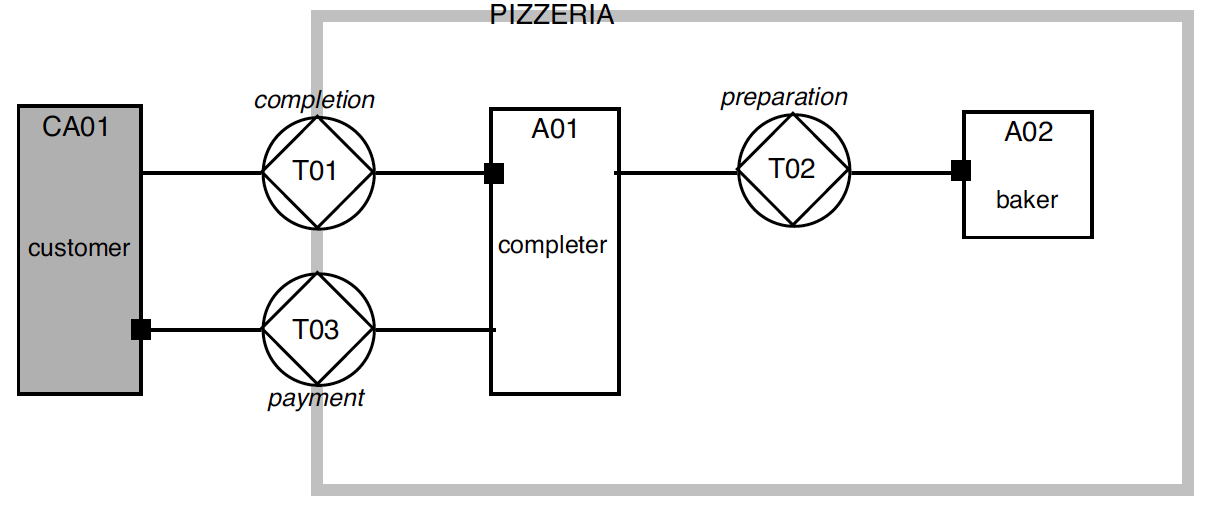
\includegraphics[scale=0.35]{obrazky/ATD-pizzeria}
\caption{ATD Pizzerie Mama Mia \cite{Dietz2006}}
\label{fig:atd_pizzeria}
\end{figure}

Pro vytváření výsledného BPMN modelu nám však bude více nápomocný Process Structure Diagram (PSD), který zachycuje všechny transakční kroky dle transakčního vzoru. V kroku 7 bude naším úkolem tyto transakční kroky vyjádřené v PSD popsat pomocí BPMN primitiv, které jsou popsány v sekci \ref{sec:tr_vzor_ulohy_signaly}.

Na \ref{fig:psd_pizzeria} můžem vidět PSD pro případ Pizzerie Mama Mia. Za povšimnutí stojí zejména šipky s přerušovaným tělem, které vyjadřují závislost vykonání C-actu na vykonání C-actu v jiné transakci. Díky tomu lze vidět, že vykonání Request T03 je závislé na Accept T02 a Execution T01 je závislá na Accept T03. Převedeno do lidské řeči to znamená, že než můžeme požádat zákazníka o zaplacení objednávky, musíme jí nejdřív připravit a zákazník ji musí akceptovat a že než je objednávka vyřízena musí dojít k jejímu zaplacení. Toto zjištění nám pomůže při vytváření BPMN modelu určit pořadí aktivit, které budeme propjovat pomocí sekvenčních toků.

\begin{figure}[H]\centering
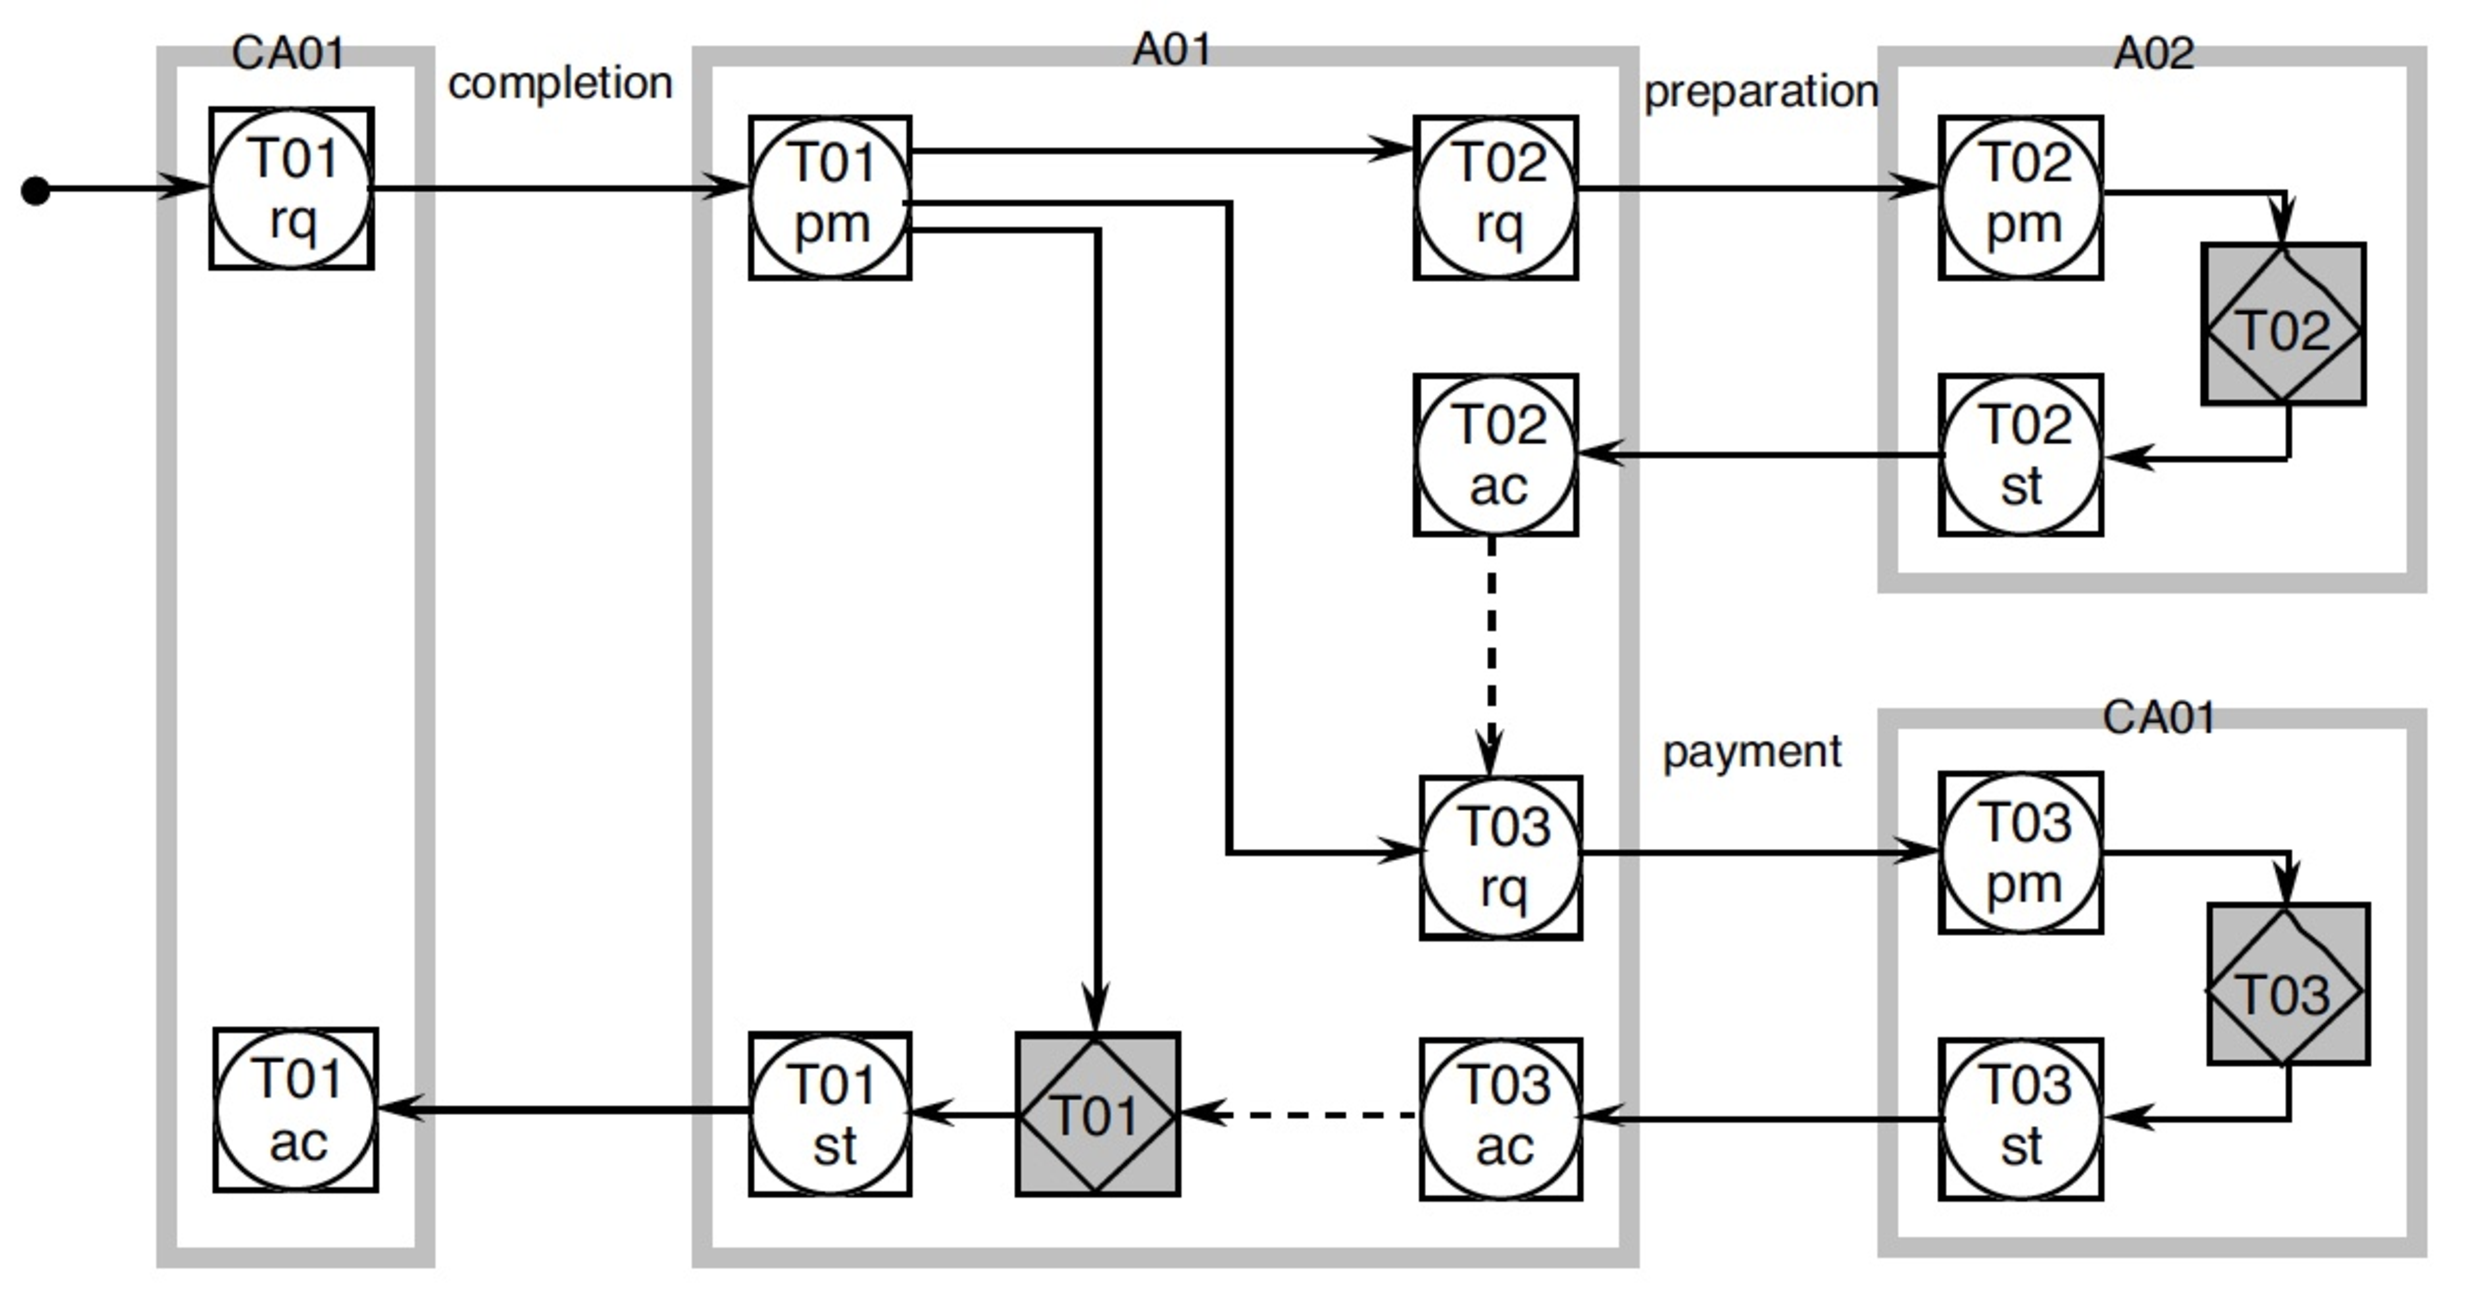
\includegraphics[scale=0.35]{obrazky/PSD-pizzeria}
\caption{PSD Pizzerie Mama Mia \cite{Dietz2006}}
\label{fig:psd_pizzeria}
\end{figure}

\subsection{Krok 7: Vytvoření BPMN modelu}
Nyní je vše připraveno pro vytvoření konečného BPMN modelu. Při jeho tvorbě budeme vycházet především z PSD modelu vytvořeného v předešlém kroce a z předpisu pro převedení transakčního axiomu do BPMN primitiv, který je uveden v sekci \ref{sec:tr_vzor_ulohy_signaly}. Postupujeme tedy po jednotlivých transakčních krocích zobrazených v PSD v obrázku \ref{fig:psd_pizzeria} a převádíme je dle tohoto předpisu do BPMN. Je důležité správně poskládat aktivity dle závislostí vyjádřených v kroku 5 i v PSD pomocí přerušovaných čar a diskutovaných v předchozím kroku.

Při vytváření PSD v předchozím kroku je použit pouze základní transakční vzor. Důvodem je větší čitelnost výsledného BPMN modelu a také absence popisu nešťastných scénářů v textovém popisu případu Pizzerie Mama Mia. Dle předpisu v sekci \ref{sec:tr_vzor_ulohy_signaly} by však nebyl problém vytvořit i BPMN model ze standardního transakčního vzoru.

Zobrazení případu Pizzerie Mama Mia v BPMN za použití metody navržené v této práci můžeme vidět na obrázku:

\begin{center}
\begin{figure}[H]
\centerline{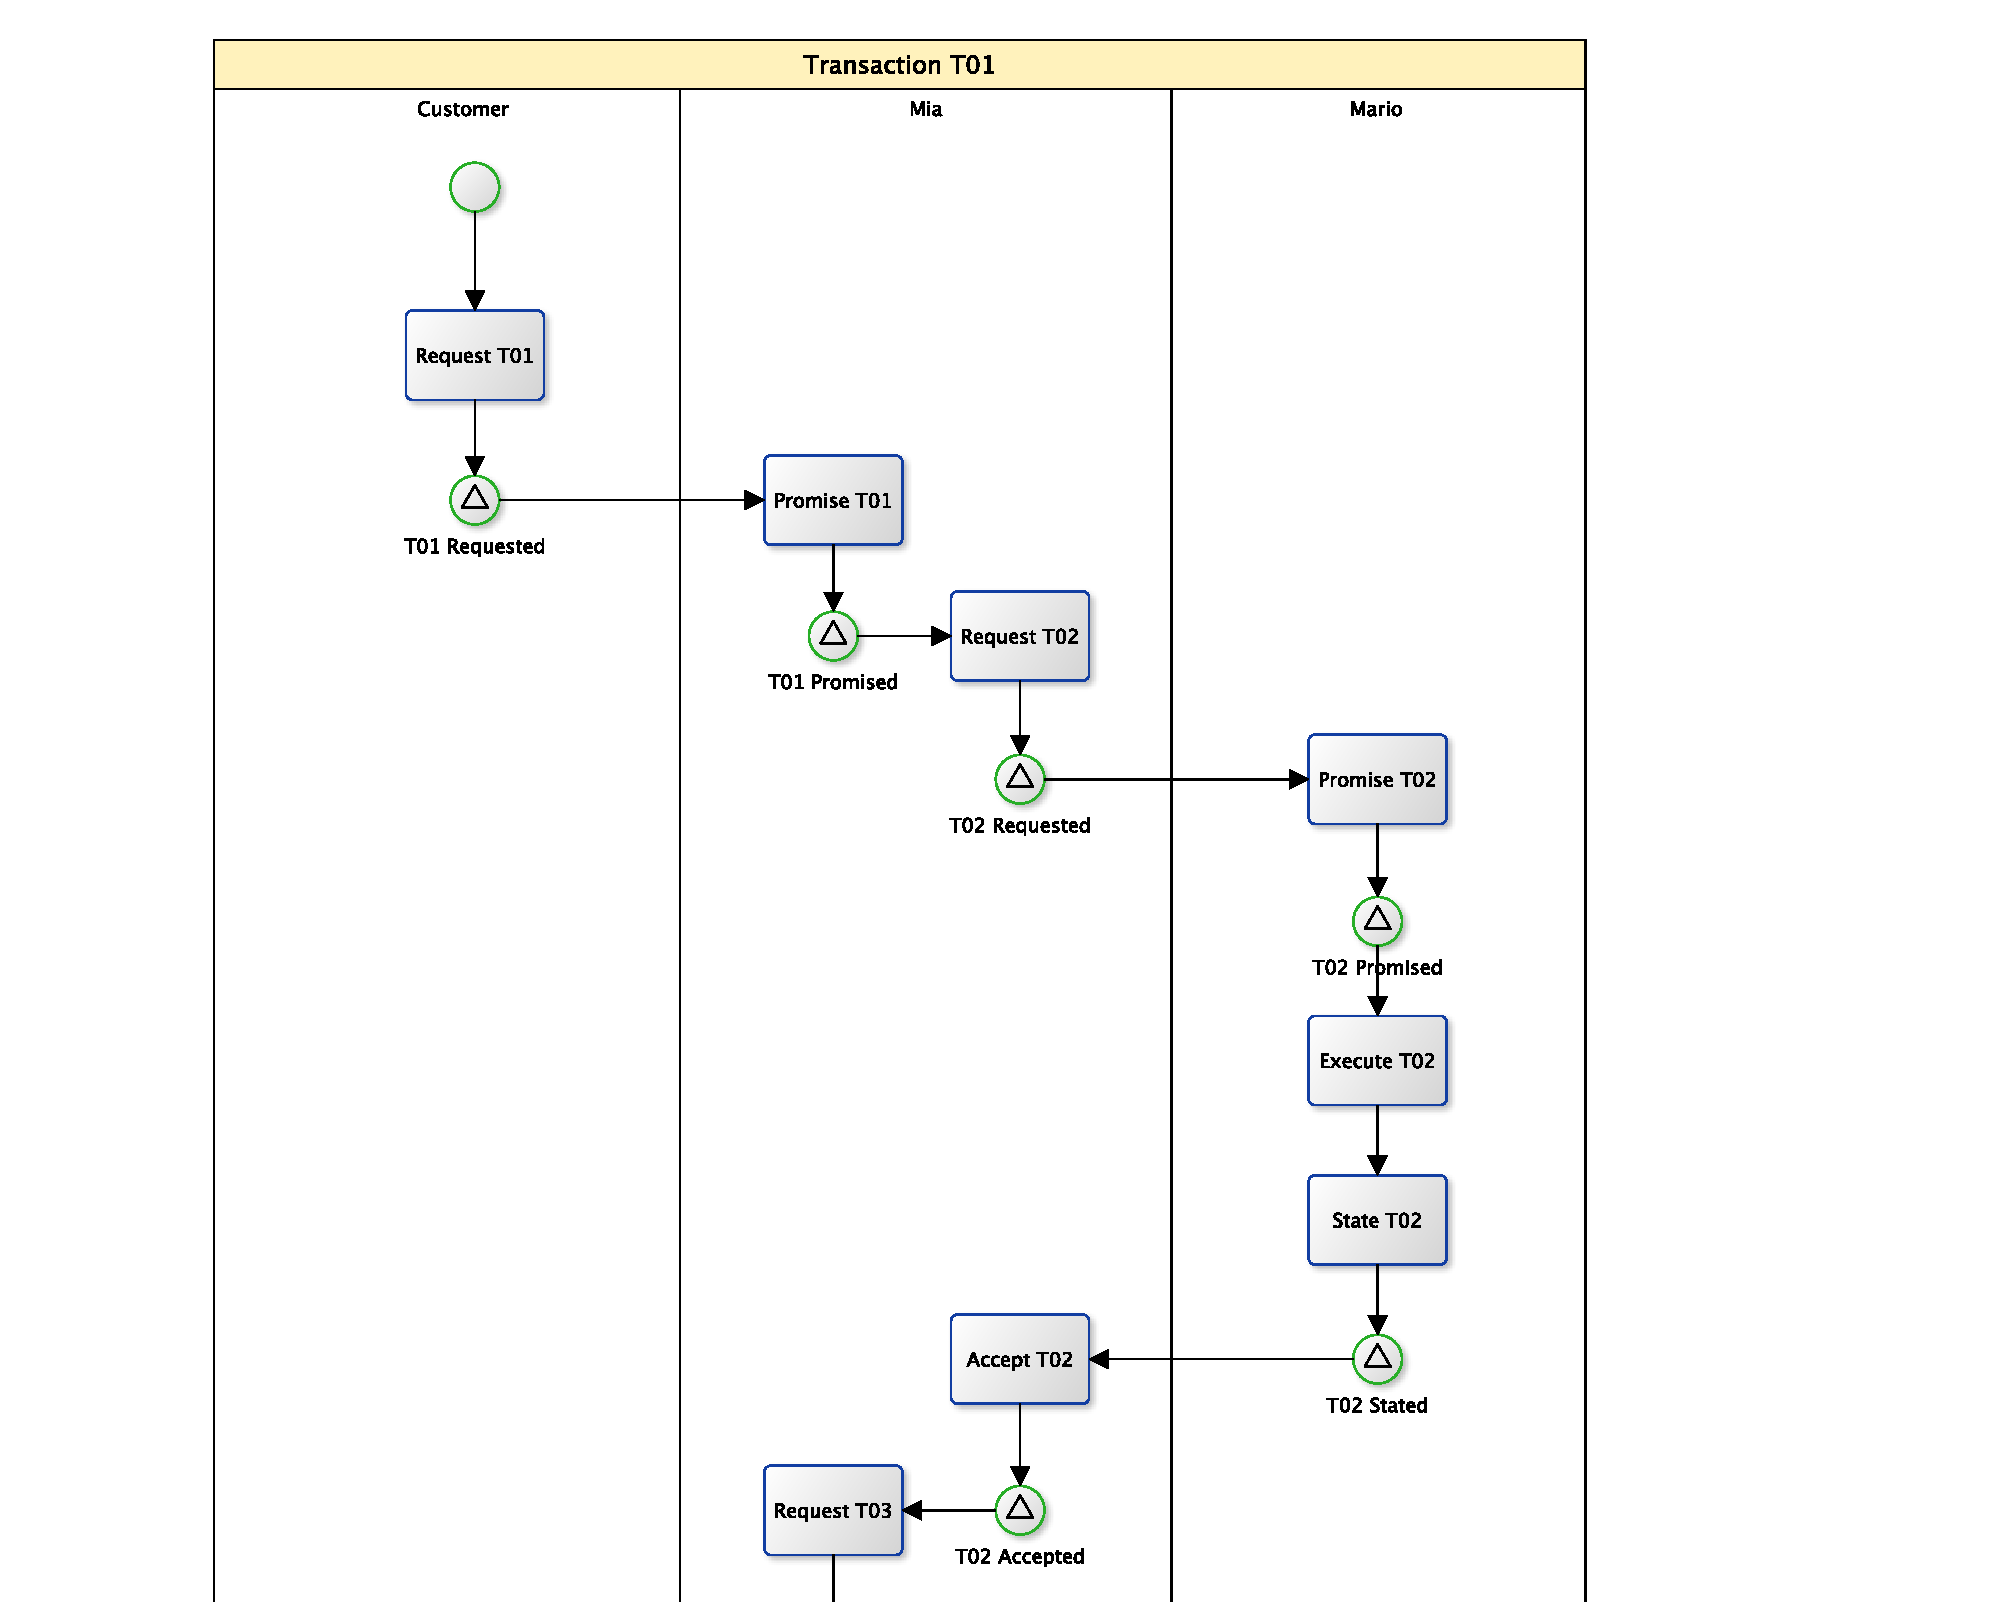
\includegraphics[width=1.28\textwidth,height=\textheight,keepaspectratio]{obrazky/pizzeria-bpmn-1}}
\caption{Případ Pizzerie Mama Mia v BPMN 1/2}
\label{fig:pizzeria_bpmn_1}
\end{figure}
\end{center}

\begin{center}
\begin{figure}[H]
\centerline{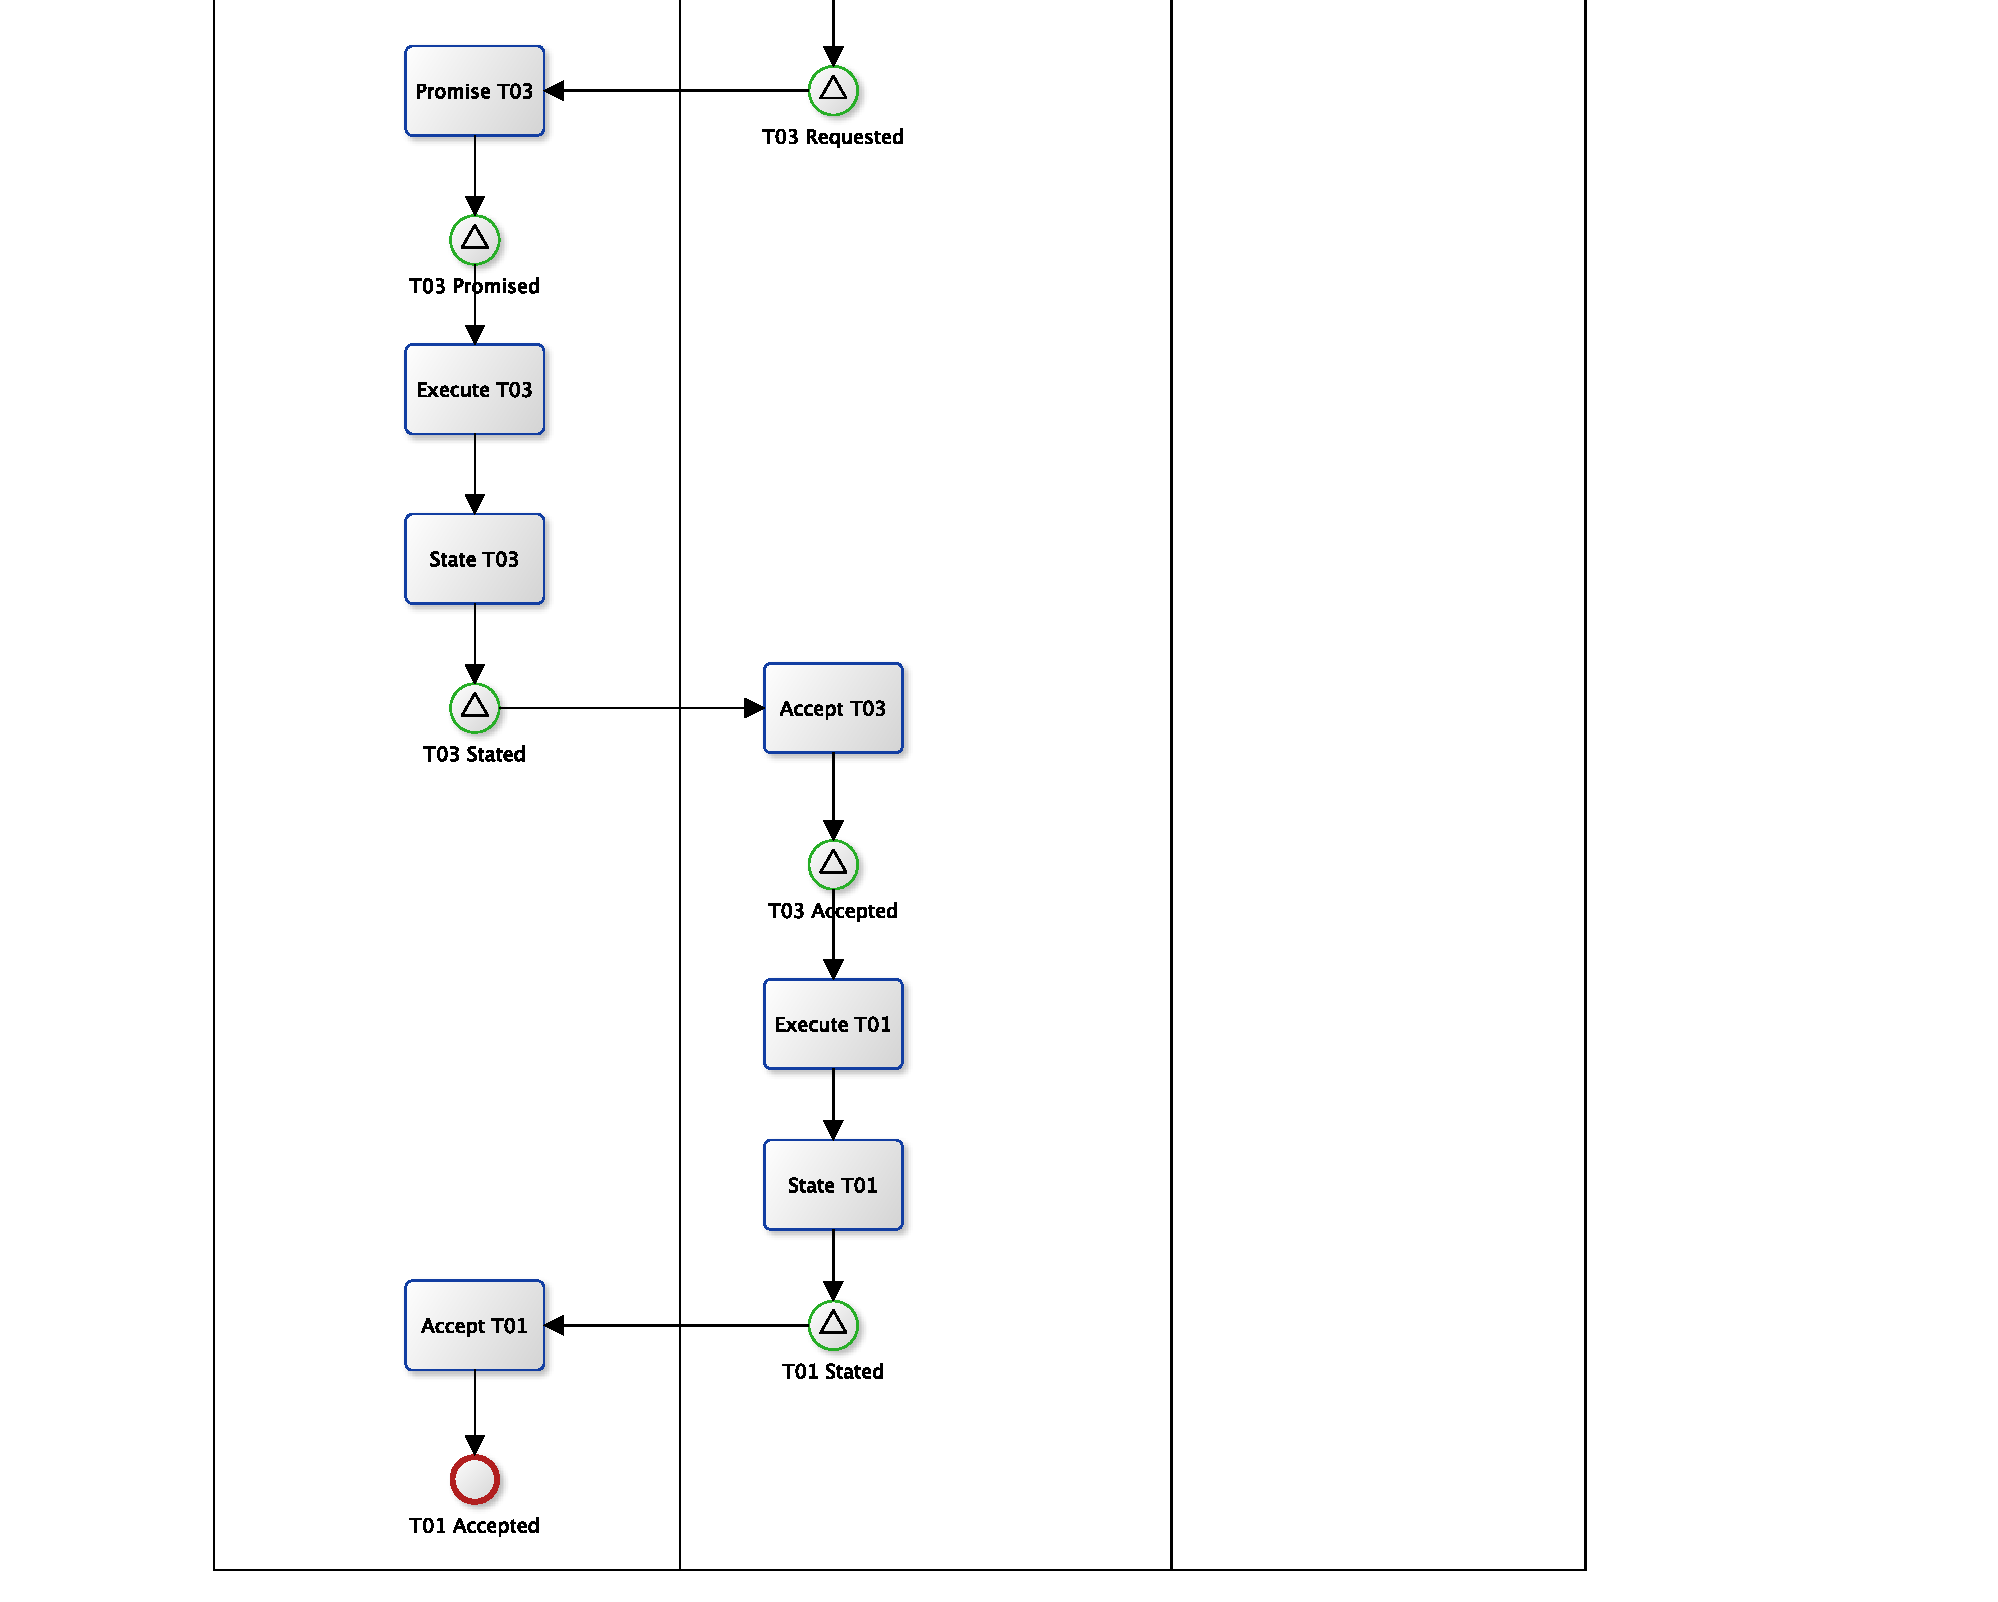
\includegraphics[width=1.28\textwidth,height=\textheight,keepaspectratio]{obrazky/pizzeria-bpmn-2}}
\caption{Případ Pizzerie Mama Mia v BPMN 2/2}
\label{fig:pizzeria_bpmn_2}
\end{figure}
\end{center}

\section{Diskuse}
Na obrázcích \ref{fig:pizzeria_bpmn_1} a \ref{fig:pizzeria_bpmn_2} vidíme, že se nám podařilo vytvořit BPMN model pro případ Pizzerie Mama Mia dle metody navržené v kapitole 5. Vytvořený BPMN model je:

\begin{itemize}
\item \textit{kompletní} dle transakčního axiomu – žádný transakční krok dle základního transakčního vzoru v modelu nechybí a díky použití plaveckých drah je jasné, který actor je zodpovědný za vykonání konkrétního transakčního kroku
\item \textit{konzistentní} dle transakčního axiomu – pořadí provádění všech transakčních kroků je konzistentní se základním transakčním vzorem
\item \textit{jednoznačný} – navržená metoda zajišťuje, že při správném aplikování všech kroků metody vznikne vždy ten samý model
\item \textit{esenciální} – výsledný model neobsahuje žádné implementační detaily. Při jeho tvorbě bylo použito pouze aktivit, které jsme vyhodnotili jako Performa.
\end{itemize}

\subsection{Slabiny metody}
\subsubsection{Modelování komplexních procesů}
Na obrázcích \ref{fig:pizzeria_bpmn_1} a \ref{fig:pizzeria_bpmn_2} jsou zachyceny pouze 3 transakce za použití základního transakčního vzoru a stejně jsme museli diagram rozdělit na 2 obrázky, protože se celý nevešel na jednu stránku. V případě modelování komplexnějších procesů, které obsahují desítky transakcí bude problém jen narůstat a model se bude obtížně vytvářet i číst.

Řešením je v tomto případě automatické generování BPMN diagramu z ATD diagramu (případně PSD dle DEMO 3) , který je mnohem méně obsáhlý a dobře čitelný i když obsahuje desítky transakcí. Pokud by bylo možné automatizovat vytváření BPMN a jejich verifikaci dle DEMO modelů, jednalo by se o velký krok dopředu.

\subsubsection{Korektní provedení kroku 2}
Z mé zkušenosti je pro velké množství lidí velmi problematické správně aplikovat krok 2 navržené metody, neboli správně provést na textovém popisu procesu Performa-Informa-Forma analýzu. Lidská řeč je totiž velmi vágní a rozdíly mezi Performa, Informa i Forma aktivitami jsou často nezřetelné a ani odborníkům se zkušenostmi s DEMO se často nedaří provést tento krok správně.

Na tomto místě je třeba uvést, že i situace, kdy se nepodaří všechny aktivity správně zařadit a jako Performa je napříkad zařazena aktivita, která Performa není, stále pravděpodobně vznikne kvalitnější BPMN model než by vzniknul neaplikováním této metody. Jak popisuje \cite{Silver2011} \uv{špatné BPMN} je dnes spíše pravidlem než výjimkou a aplikace navržené metody by tedy za každých okolností přispěla obecně k lepším výsledkům.

\nocite{*}
\bibliographystyle{plain}
\bibliography{Bibliography}

\end{document}